\section{Memory allocation and deallocation}
\label{sec:memory-alloc-deall}

Although it is not strictly necessary to write Java programs, a basic
understanding of how memory is managed in Java will help you become a
better programmer. 

At this point, you already know a bit 
about how Java stores the data of your 
program in your computer's memory. You know that local variables of
simple types are stored in the stack while objects are stored in
the heap (with pointers pointing to them). 
You also know that the stack adds a new level every time a
new method is called, and that variables on that level are forgotten
as soon as the method terminates. You know as well that objects 
contain data in them, sometimes simple types and sometimes complex
types, i.e.~pointers to data in other objects. 

The memory of a computer is finite. If it was used but never released,
the computer would run out of memory even with the simplest of
programs. Using memory is easy: declaring variables, creating new
objects\ldots all those operation use new memory. How is this memory
released so that it can be used again by the same or other programs?

\subsection{Using and releasing memory in the stack}
\label{sec:using-rele-stack}

As you already know, the stack is where the variables of simple types
are stored. It is also the place where the computer stores the
pointers for the complex types. 

Every time a variable declaration statement is executed, 
a small ``box'' is used in the
stack to hold its value; this ``box'' is tagged
with a name and a value. It is important to note that memory is not
used until the variable is declared, i.e.~until the statement where
the variable is declared is reached. A program can declare many
variables in different methods, but until those methods are executed
the variables do not use any memory ---actually, they do not exist. 

\begin{verbatim}
    // Some examples of variable declaration
    // Simple types: the box contains the data
    int count;
    double exchangeRate;
    // Complex type: the box is only a pointer to where the data really is
    String familyName;
    Person john;
\end{verbatim}

As you know, in Java the type is set once 
and cannot change afterwards.
%%%%%%%%%%%%%%%%%%
%, except with a special operation called \emph{casting}. %% NOT TRUE:
%  % casting changes the type of values, but not variables. 
%%%%%%%%%%%%%%%%%%
In other languages, such as Groovy, the type
can change over time. 

When a new method is called, a new ``level'' is added to the stack. The
variables declared for the new method (starting with the 
method's parameters themselves)
are stored on the new level of the
stack (see Figure~\ref{fig:stackparameter}). 
When the method ends, usually because the \verb+return+
statement is reached, the variables are forgotten and the memory they
were using is released. That memory can then be used for variables of
other methods.

\begin{figure}[bhtp]
  \centering
  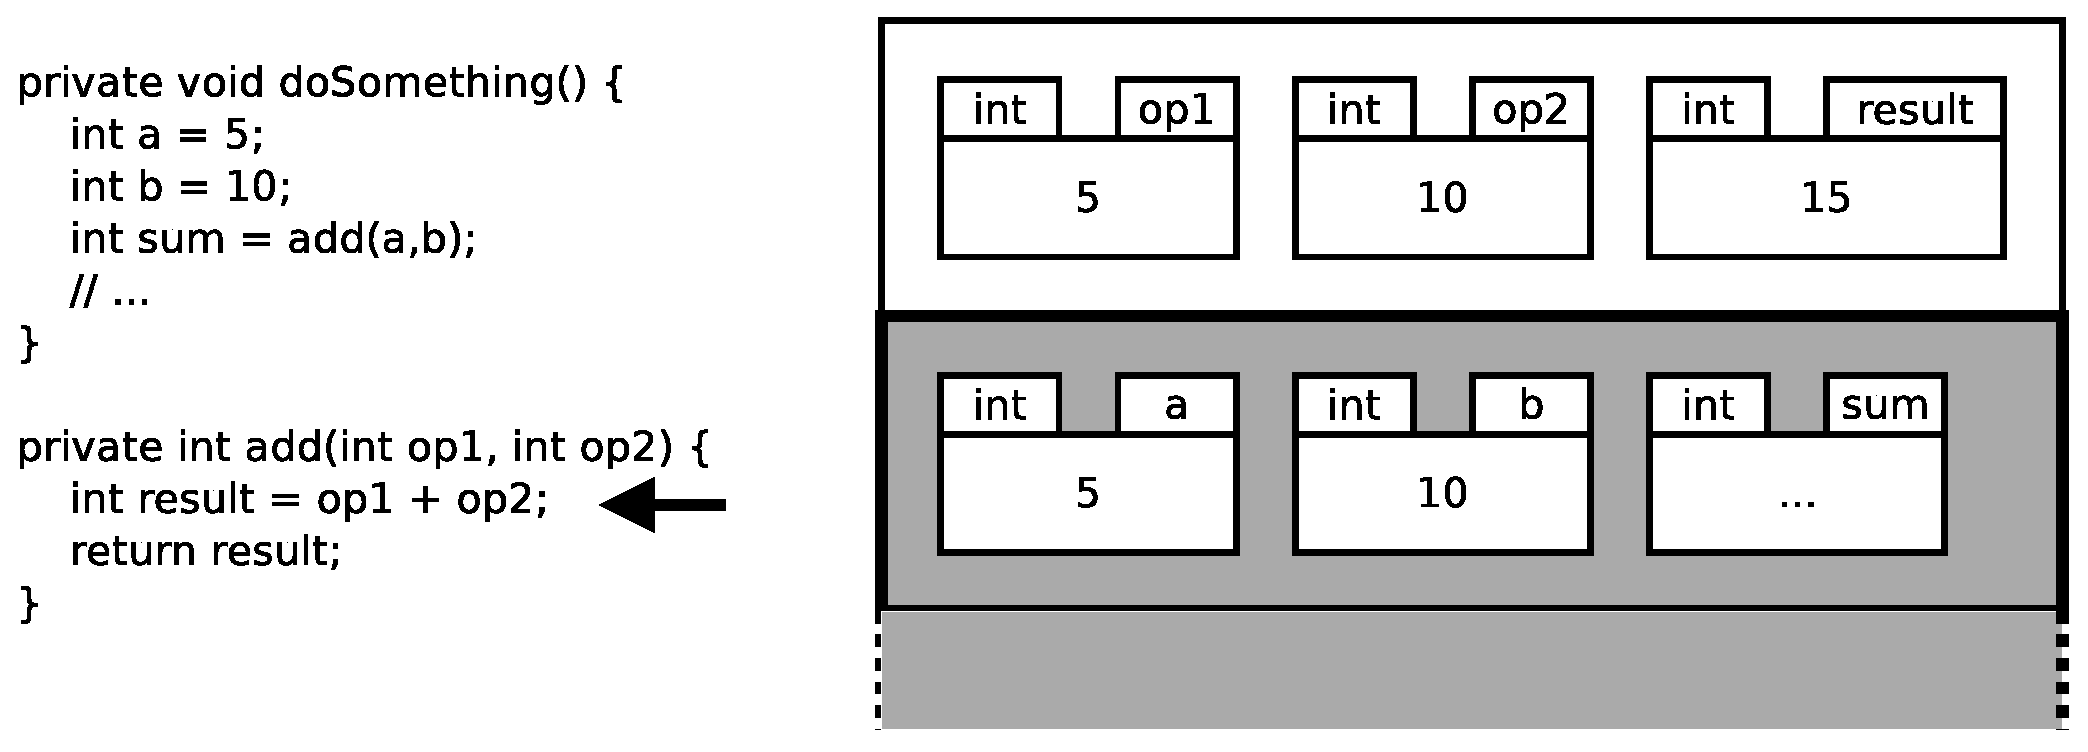
\includegraphics[width=\textwidth]{gfx/parameter-stack}
  \caption{When a method (add) is called, a new level is put on the
    stack to store the parameters and the local variables. While in
    the method, the variables of the other method (a, b, sum) cannot
    be accessed: they are on a different level of the stack, and only
    the most recent one is accessible. Note that if those variables
    were of complex types, their ``boxes'' would be pointers pointing
    to objects in the heap. Note also that we do not know the value
    stored in ``sum'' until the method ``add(int,int)'' returns a
    value (the arrow marks the current statement being executed).}
  \label{fig:stackparameter}
\end{figure}

This is not the whole story, as you know. Some of the variables can
be of complex types, which means that they use memory in the
heap. Moreover, this memory used in the heap is not automatically
forgotten or released when the method ends: objects remain in memory,
and this is how changes to complex types can survive the scope of a
method. But how is memory released in the heap?

\subsection{Using and releasing memory in the heap: Garbage collection}
\label{sec:garbage-collection}

In order to store new data in the heap, we use the keyword
\verb+new+. This keyword reserves some portion of memory in the heap,
enough to hold an object of the right type, and then makes the pointer
in the stack point to the object in the heap. The memory used by the
object will remain used by the program (and by nobody else) until it
is released. 

In some languages, like C or C++, the programmer must release the
memory manually. Although this allows very good programmers to produce
very efficient programs, it is a big source of bugs and errors because
programmers are human and have a tendency to forget to release the
memory they have used, or to release it more than once. This
is why most modern languages, including Java, assume the
responsibility of releasing the memory when it is no longer
used. Computers are better than humans at doing this sort of clerical
work. 

Java includes a little program that operates ``behind the scenes''
called the \emph{garbage collector}. This program keeps an eye on the memory
of the computer\footnote{Strictly speaking, it only observes the
  memory of the Java Virtual Machine, not the whole physical memory of
the computer.}, looking for objects that are no longer necessary in order
to release the memory they are using. 

How does the garbage collector know when an object is no longer
necessary? Because it is \emph{unreachable}. 

We know that variables of complex types are just pointers to
objects. We also know that there can be many pointers pointing to the
same object. This happens every time you call a method with a complex
parameter: as the parameters' values are copied when a method is
called, there are always two pointers to every object that is
giving as parameter. 

\begin{figure}[bhtp]
  \centering
  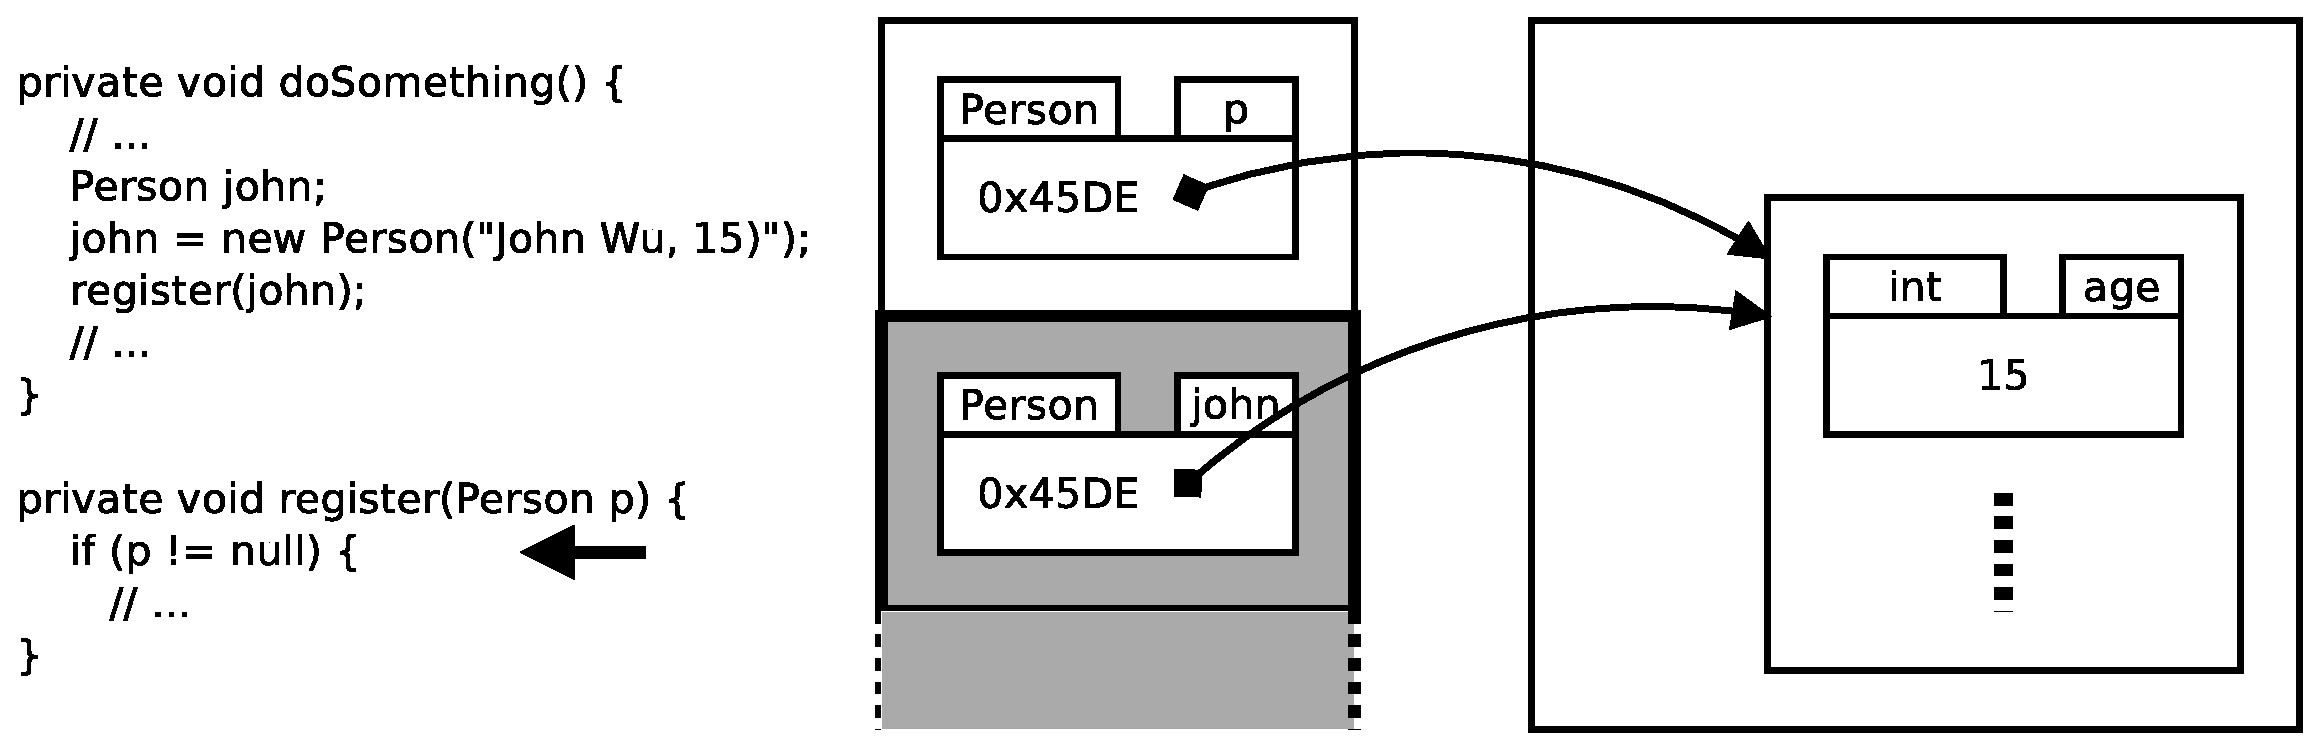
\includegraphics[width=\textwidth]{gfx/parameter-stack-2}
  \caption{When a method is called, the values of the parameters are
    copied on the stack. If the parameters were of complex types, this
    results in a new pointer pointing to those objects given as
    parameters.}
  \label{fig:padfsajdghshdg}
\end{figure}

In the same way, an object may end up with no pointer pointing to
it. This happens when you delete an object from a linked list, for
example. An object with no pointer pointing to it is unreachable: it
can never again be accessed by your program, no matter how hard you
try. 

\begin{figure}[hbtp]
  \centering
  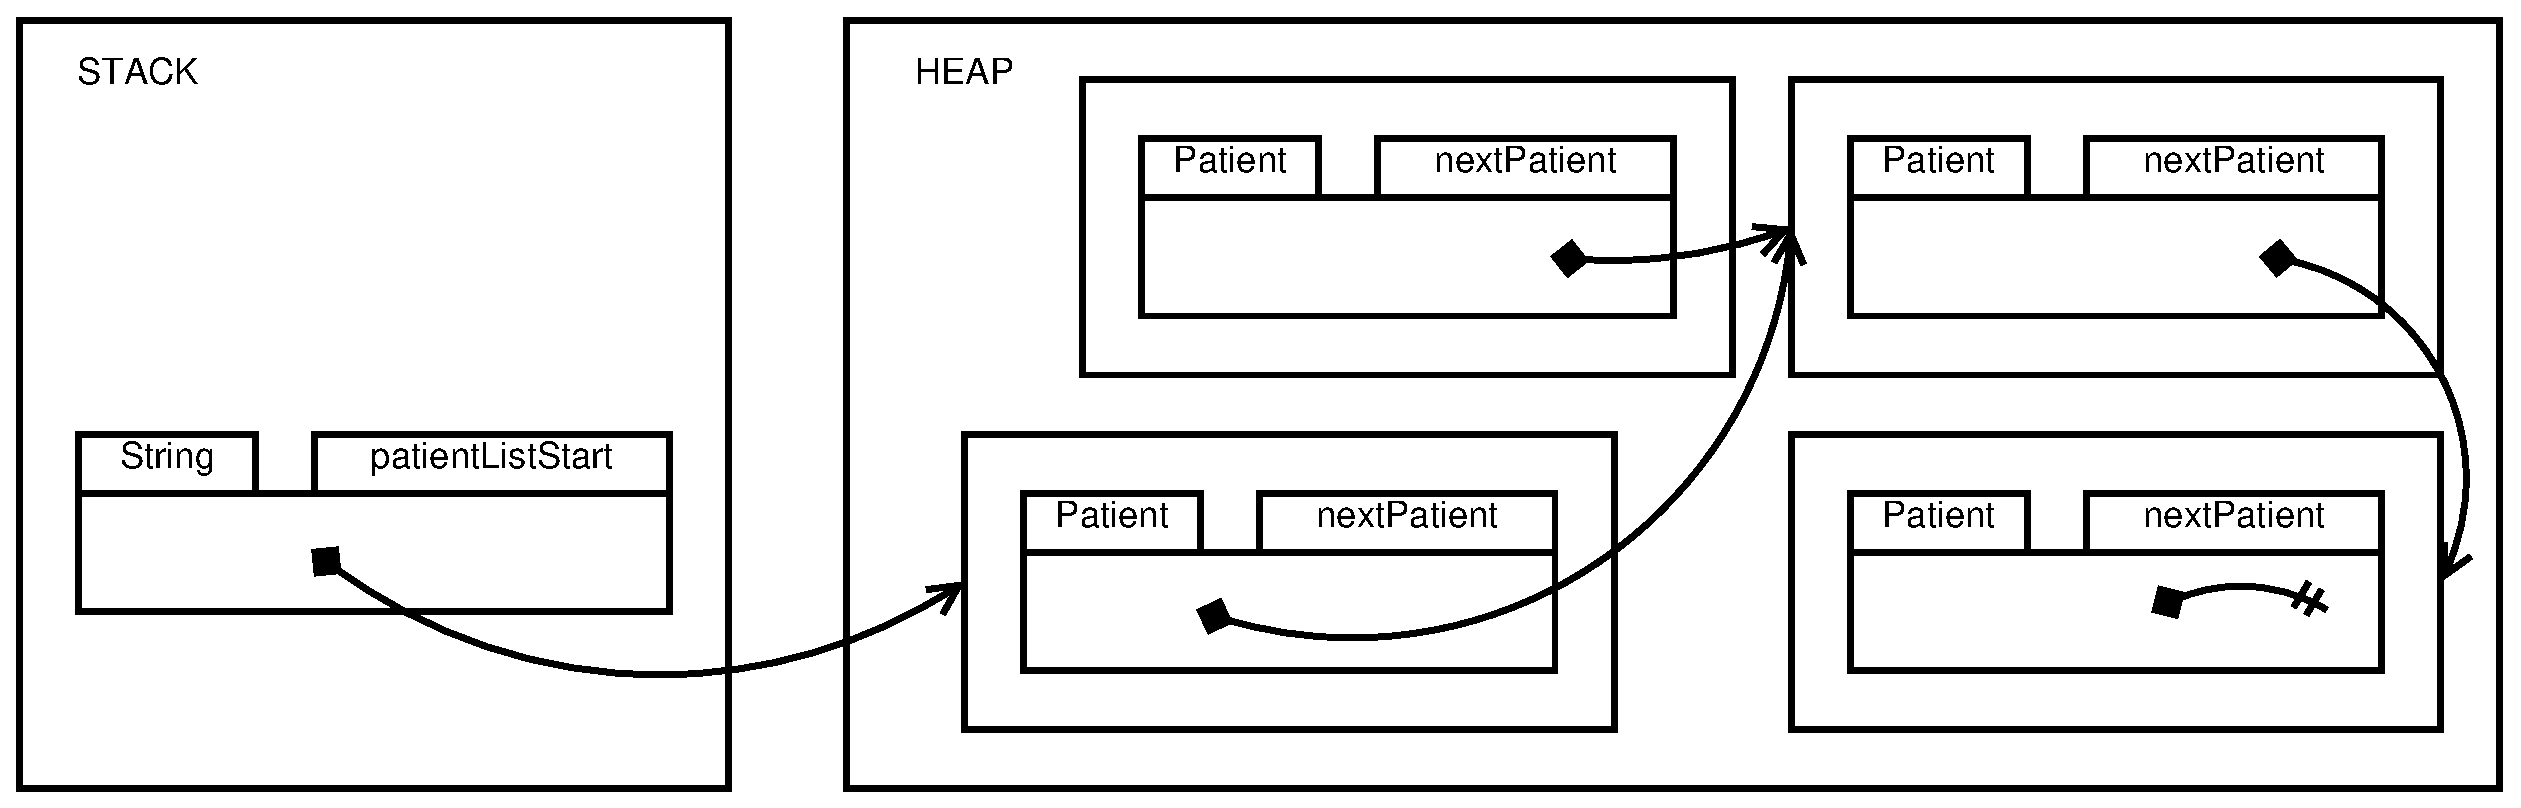
\includegraphics[width=\textwidth]{gfx/lists-remove-2}
  \caption{Deleting elements of a dynamic list means changing a pointer
    to point to a different element, resulting in the deleted element
    becoming unreachable.}
  \label{fig:padfsajdg4g}
\end{figure}

\begin{figure}[hbtp]
  \centering
  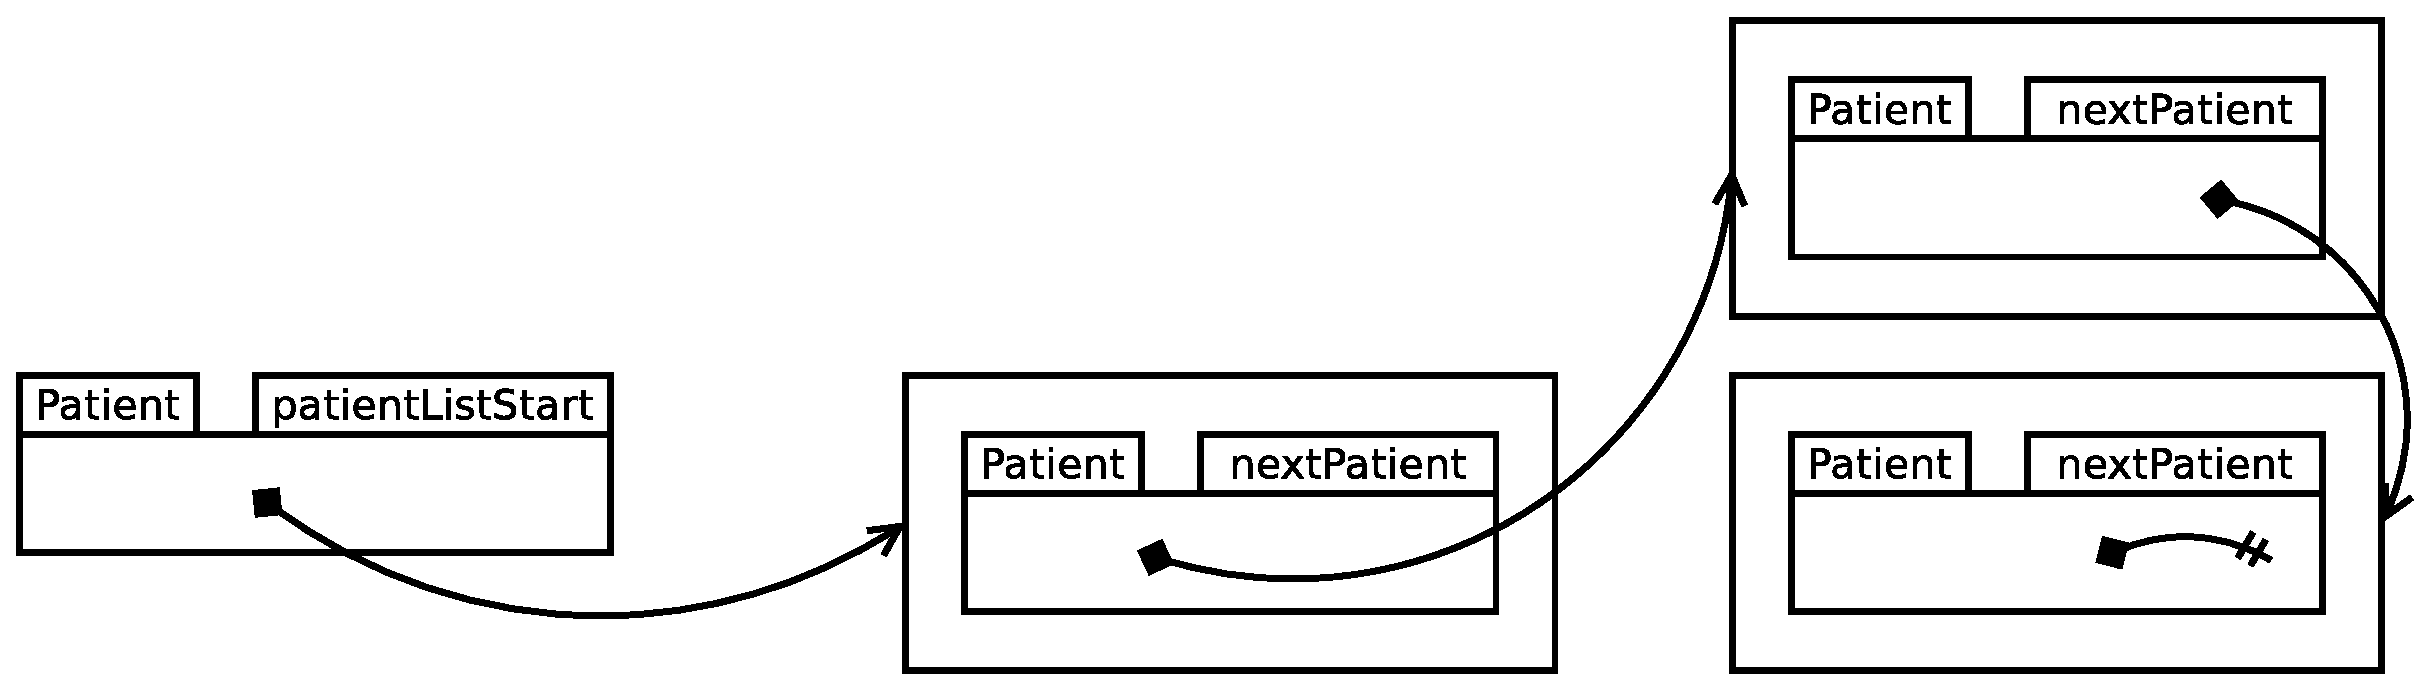
\includegraphics[width=\textwidth]{gfx/lists-remove-3}
  \caption{The garbage collector detects unreachable objects and
    releases the memory they use. The memory is then available for new
    objects.}
  \label{fig:padfsajdg4eg}
\end{figure}



The garbage collector is not running all the time, because that would
use too many resources. It is usually dormant, and wakes up when the
memory starts to get full. Then it looks around in the memory for
unreachable objects. When it finds one, it releases the memory used by
it, and now it can be used by other objects. 

% TODO figure